
\chapter{Динамічні акустоіндуковані ефекти в опромінених та неопромінених кремнієвих структурах з p--n переходом}
\section{Кремнієві сонячні елементи та режими їх радіаційного опромінення\label{SSC}}
Сонячні елементи, які досліджувалися в роботі, були створені на основі пластин кремнію діаметром близько 100~мм (радіус дорівнював 2 дюйми).
Пластини вирізані були вирізані зі злитків, вирощених за методом Чохральського, мали товщину 300~мкм і були орієнтовані в напрямі $<$111$>$.
Легування здійснювалось шляхом додавання у розплав атомів бору (КДБ10).
Концентрація основних носіїв заряду $p_p=1,4\cdot10^{15}$~см$^{-3}$.
% та $p_p=4.5\cdot10^{15}$~см$^{-3}$).

Для створення n$^+$ емітера проводилась імплантація іонів фосфору, після закінчення якої було проведено активізуючий відпал.
Як наслідок, був створений шар з електронною провідністю товщиною близько  0,5~мкм з концентрацією вільних носіїв заряду $10^{19}$~см$^{-3}$.

Поверхня пластини була пасивована шляхом нанесення плівки Al$_2$O$_3$.
Крім того, на фронтальну поверхню був нанесений антивідбиваючий шар діоксиду титану (TiO$_2$) з використанням методу APCVD (atmospheric pressure chemical  vapour  deposition)
З використанням методу трафаретного друку (screen printing) було створено омічні алюмінієві електроди (суцільний на задній поверхні та металева сітка на передній).
Нарешті, був проведений швидкий відпал отриманих структур при температурі $800^\circ$C тривалістю декілька хвилин.
Структура досліджених сонячних елементів зображена на Рис.~\ref{figSSC},а.
Зауважимо, що цей рисунок наведено без збереження масштабних співвідношень між окремими частинами.

Для досліджень використовувалися зразки площею $1,5\div2,1$~cm$^{2}$, вирізані з різних (переважно центральних) областей пластини.
Для позначення зразків надалі використовується запис на кшталт SSC$x$, де $x$ --- номер зразка.
Місце розташування зразків на вихідній пластині показано на Рис.~\ref{figSSC},б.


\begin{figure}
\center
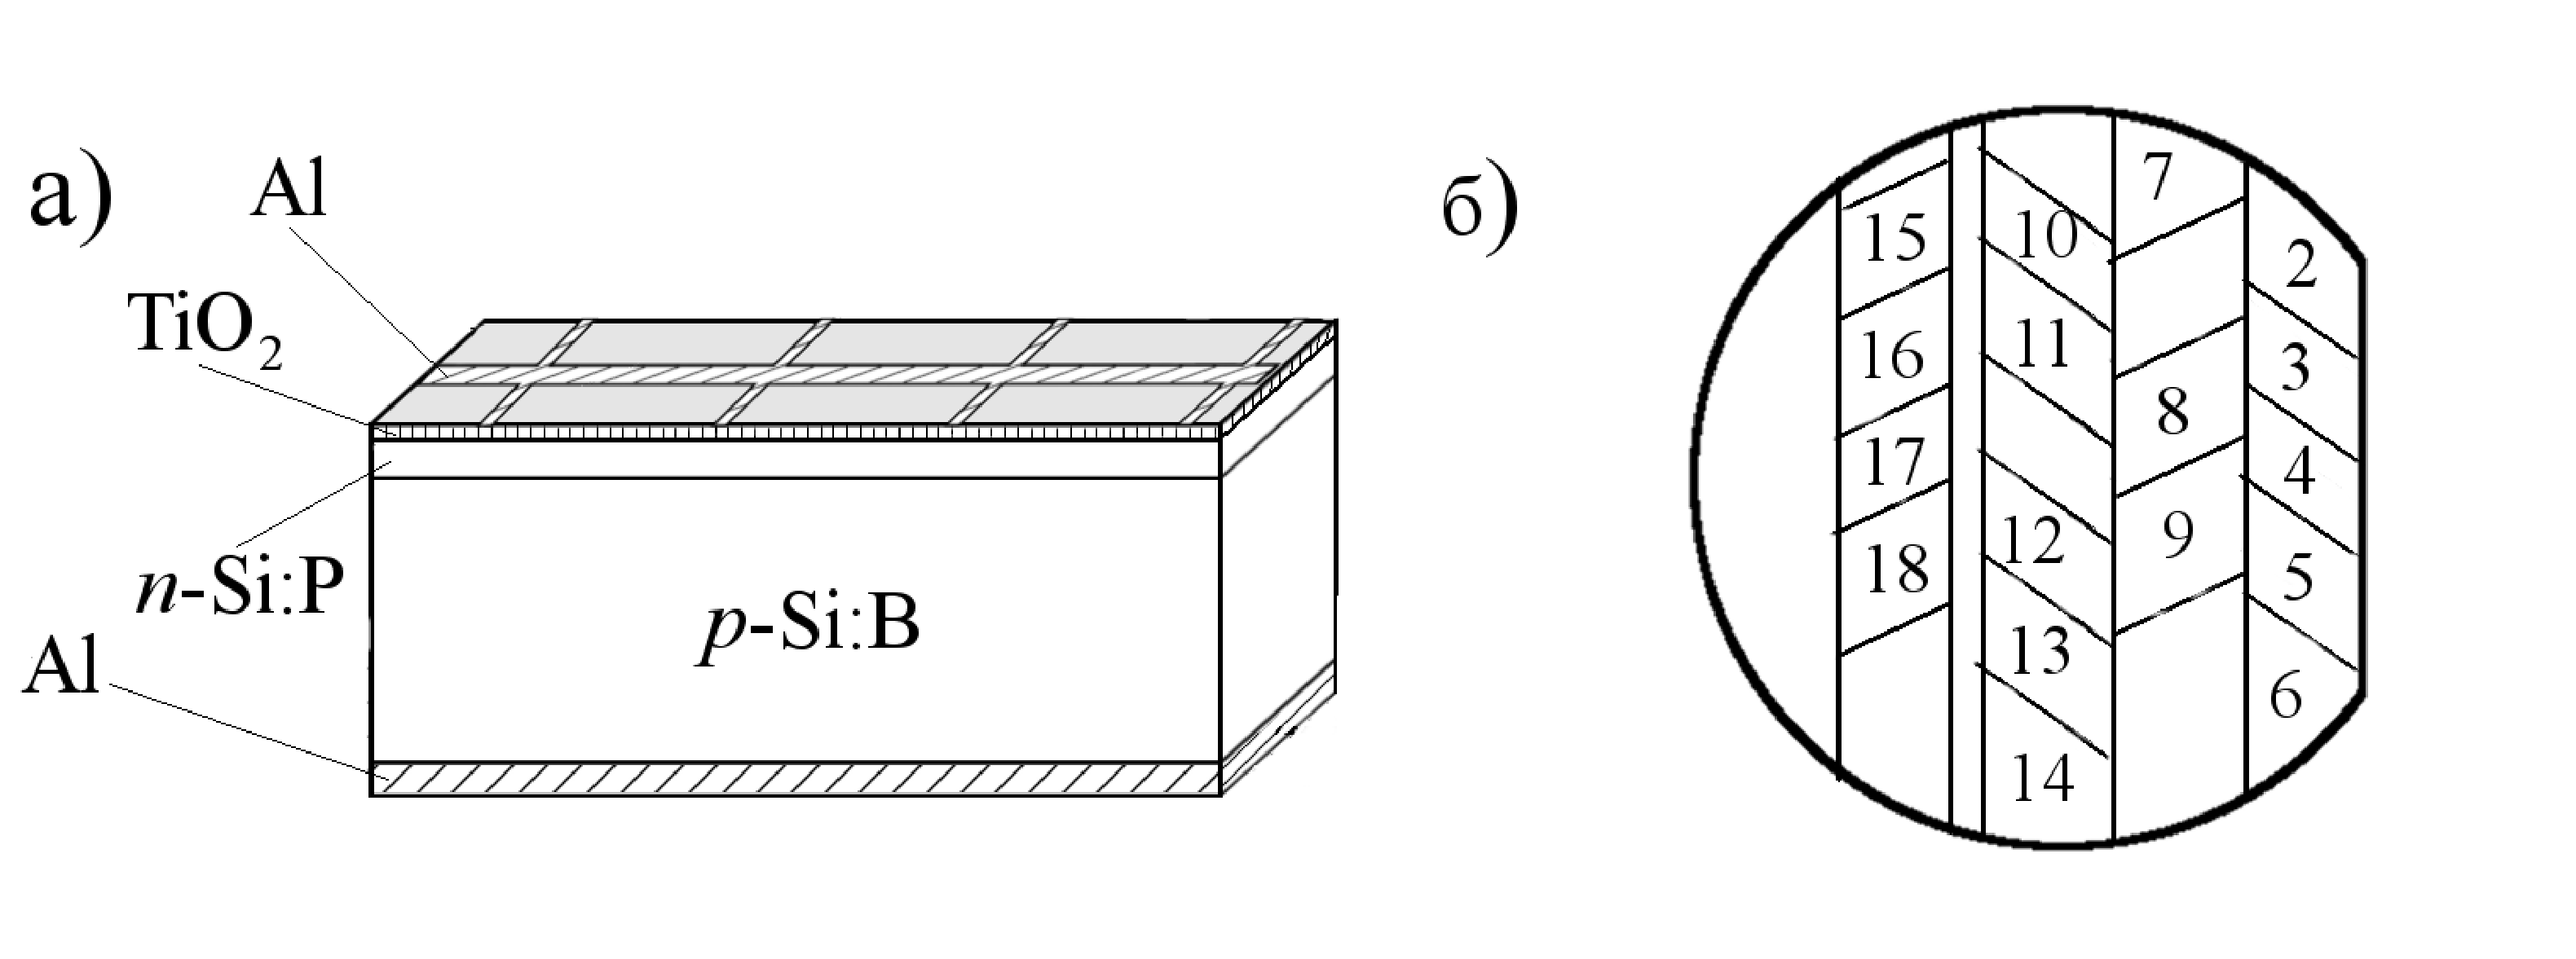
\includegraphics[width=1.0\textwidth]{SSC}%
\caption{\label{figSSC}
Структура кремнієвих сонячних елементів (а) та місце розташування зразків (б).
}
\end{figure}


